\documentclass[12pt]{article}
\usepackage{amsfonts}
\usepackage{comment}
\usepackage{tikz}
\usetikzlibrary{arrows,automata}
\begin{document}

\noindent
Jason Downing \\
Email: jason\_downing@student.uml.edu \\
Foundations of Computer Science \\
Homework \#2 - Chapter 1: DFA, NFA\\
10/6/2016 \\

\noindent
1.3 \\
The formal description of a DFA M is \\
\{q1, q2, q3, q4, q5 \}, \{u, d\}, $\delta$, q3 , \{q3\}, \\
where $\delta$  is given by the following table:
\begin{center}
\begin{tabular}{ c | c c }
 & u & d \\
\hline
 q1 & q1 & q2 \\ 
 q2 & q1 & q3 \\  
 q3 & q2 & q4 \\
 q4 & q3 & q5 \\
 q5 & q4 & q5
\end{tabular}
\end{center}

\noindent
Give the state diagram of this machine.	\\

\noindent
Initial state is q3, so that is where the machine will start. \\
We can use the table to create the nodes, and connect them as needed. \\
The accepted state is q3 so we will mark that with a double circle to \\
show that as the accepted state of the machine. \\

\begin{center}
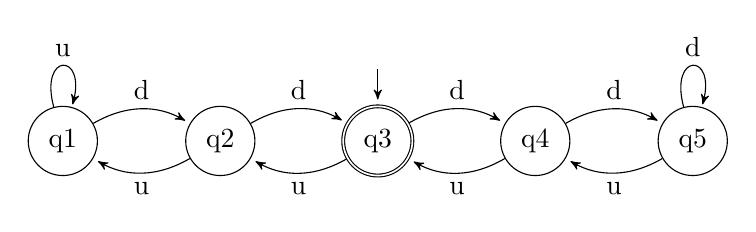
\begin{tikzpicture}[>=stealth',shorten >=2pt, auto, node distance=2cm]
	% Nodes {q1, q2, q3, q4, q5}
	\node [state] 	(q1) 				{q1};
	\node [state] 	(q2) [right of=q1]  {q2};
	\node [state, initial, initial text=, initial where=above, accepting]  (q3) [right of=q2]  {q3};
	\node [state]	(q4) [right of=q3]  {q4};
	\node [state]   (q5) [right of=q4]  {q5};

	% Paths	{{1, 2}, {2, 3}, {1, 3}, {2, 4}, {1, 4}}
	\path [->] 	(q1) edge [loop above] node	{u}	(q1)
	            (q1) edge [bend left]  node {d} (q2)
				(q2) edge [bend left]  node {u} (q1)
				(q2) edge [bend left]  node {d} (q3)
				(q3) edge [bend left]  node {u} (q2)
				(q3) edge [bend left]  node {d} (q4)
				(q4) edge [bend left]  node {u} (q3)
				(q4) edge [bend left]  node {d} (q5)
				(q5) edge [bend left]  node {u} (q4)
				(q5) edge [loop above] node	{d}	(q5);
				
\end{tikzpicture} \\
\end{center}


\noindent
1.4: a, c, e, f, g \\


\noindent
1.5: c, d, e, f, g, h \\


\noindent
1.6: a, b, c, d, e, f, g, h, I, j, k, l, m, n \\


\noindent
1.7: b, c, d, e, g, h \\


\noindent
1.8: a, b \\


\noindent
1.9: a, b \\


\noindent
1.10: a, b, c \\


\noindent
1.12 \\


\noindent
1.13 \\

\noindent
1.16 \\

\noindent
1.17: a, b \\

\noindent
1.18 \\

\noindent
1.20: a, b, c, d, e, f, g, h \\

\noindent
1.21 \\

\noindent
1.22 \\

\end{document}